% CSE Seminararbeit
% Thema: Ein auf Neuronalen Netzen basierendes Ensemble-Modell zur Windprognose
% Autoren: Alicia Pirwass, Daniel Müller

\documentclass[
12pt, %Schriftgröße
toc=listofnumbered, %Tab.- & Abb.verzeichnis ins TOC
toc=chapterentrydotfill, %TOC: Punkte auch nach Kapitel
numbers=noenddot, %Kapitelüberschrift: Kein Endpunkt z.B. 2.2. --> 2.2
captions=tableheading, %Mehr Platz bei Captionüberschriften (Tabelle)
]{scrreprt}


%%%%% SCHRIFTSATZ, SPRACHE, SCHRIFTART
\usepackage[T1]{fontenc}
\usepackage[ngerman]{babel}
% Nur mit LuaTex Interpreter nutzbar
%\usepackage{mathfont} % Dieses Packet läd auch fontspec
%\setmainfont{Segoe Pro} % Textschrift separat setzen


%%%%% INHALTSVERZEICHNIS
%\setuptoc{toc}{numbered} % TOC ins TOC, benötigen wir hier nicht 
%\addtokomafont{chapterentrypagenumber}{\normalfont\textbf}

\addtokomafont{disposition}{\rmfamily}
\addtokomafont{chapterentry}{\textbf}
\RedeclareSectionCommand[tocnumwidth=2.5em]{chapter}
\RedeclareSectionCommand[tocnumwidth=2.5em,tocindent=2.5em]{section}
\RedeclareSectionCommand[tocnumwidth=2.5em,tocindent=5em]{subsection}
%\newcounter{romanchapter} Benötigen wir nur, wenn z.B. Abstract, Literaturverz. und Anhang römisch nummeriert werden soll


%%%%% MATHEMATIK
\usepackage{amssymb, amsmath}
\usepackage{isomath}


%%%%% BIBLIOGRAPHIE
\usepackage[style=ieee, mincitenames=1, maxcitenames=1]{biblatex}
\usepackage{url} % Damit URLs in der Quelle schön umgebrochen werden
\setcounter{biburllcpenalty}{7000} % Einstellungen für Packet url
\setcounter{biburlucpenalty}{8000} % Einstellungen für Packet url
\DefineBibliographyStrings{ngerman}{andothers = {{et\,al\adddot}},}
\addbibresource{bib.bib} %
\usepackage{csquotes}
%\emergencystretch=1em
\usepackage[final]{microtype}
%\usepackage[expansion, final]{microtype}
%\usepackage{natbib}
%\setcounter{biburlnumpenalty}{9000}
%\setcounter{biburllcpenalty}{9000}
%\setcounter{biburlucpenalty}{9000}


%%%%% ANHANG
\usepackage{appendix}


%%%%% FARBEN
\usepackage[table,xcdraw]{xcolor}
\definecolor{color20}{RGB}{35,35,35}
\definecolor{color25}{RGB}{69,69,69}
\definecolor{color30}{RGB}{80,80,80}
\definecolor{color80}{RGB}{190,190,190}


%%%%% ÜBERSCHRIFTEN DER EBENEN ÄNDERN
\addtokomafont{chapter}{\color{color30}\normalfont\textbf}
\addtokomafont{section}{\color{color30}\normalfont\textbf}
\addtokomafont{subsection}{\color{color30}\normalfont\textbf}
\addtokomafont{caption}{\small\color{color30}\textit}
\addtokomafont{captionlabel}{\small\color{color30}\textit}


%%%%% LAYOUT
\usepackage[left=2cm,right=2cm,top=3cm,bottom=3cm]{geometry}
\setlength\parindent{0pt} %Kein Einzug nach Ebenenbeginn
\usepackage[onehalfspacing]{setspace} %Zeilenabstand 1,5
\RedeclareSectionCommand[beforeskip=20pt,afterskip=20pt]{chapter} %Wenn neues Chapter startet, gehts auf ne neue Seite. Damit Abstand zur Kopfzeile nicht zu groß, beforeskip = 20
\usepackage[justification=justified,labelfont=bf,format = plain]{caption}


%%%%% KOPF- & FUẞZEILE
\usepackage[headsepline,automark]{scrlayer-scrpage}
\pagestyle{scrheadings}
\clearscrheadfoot
\clearscrplain 
\ihead{\headmark}
\ofoot{\pagemark}
\renewcommand*\chapterpagestyle{scrheadings} %K.&F.zeile auch bei Chapterbeg.


%%%%% BILDER
\usepackage{graphicx}
\usepackage[export]{adjustbox}
\usepackage[section]{placeins}
\let\Oldsection\section
\renewcommand{\section}{\FloatBarrier\Oldsection}
\let\Oldsubsection\subsection
\renewcommand{\subsection}{\FloatBarrier\Oldsubsection}
\let\Oldsubsubsection\subsubsection
\renewcommand{\subsubsection}{\FloatBarrier\Oldsubsubsection}
%\usepackage{here} % mit H in includegrafix wird Bildpos gezwungen


%%%%% TABELLE
\usepackage{multirow}
\usepackage{tabularx} % Nachfolgende 3 Befehle, damit Tabellen Spaltengröße definiert werden kann. z.B. nicht mehr {ccc} sondern {C{2cm}C{2cm}C{2cm}}, Folgende befehle zur neudefinierung:
\newcolumntype{L}[1]{>{\raggedright\arraybackslash}p{#1}}
\newcolumntype{C}[1]{>{\centering\arraybackslash}p{#1}}
\newcolumntype{R}[1]{>{\raggedleft\arraybackslash}p{#1}}
\usepackage{longtable} %Mehrseitige Tabellen (Abkürzungsverz.)
\setlength{\tabcolsep}{0.5em} % for the horizontal padding
\renewcommand{\arraystretch}{1.2}% for the vertical padding


%%%%% QUICK COMMANDS
\newcommand{\WY}{Weyarn }
\newcommand{\qm}[1]{\glqq#1\grqq{}} %Anfzeichen
\newcommand{\gradC}[1]{#1$^\circ C$}
\newcommand{\abs}[1]{\lvert #1 \rvert}
\newcommand{\highlight}[1]{\textbf{\textcolor{red}{#1}}}
\newcommand{\finalize}[1]{\textcolor{red}{#1}}

%%%%% VERLINKUNG
\usepackage[hidelinks,hypertexnames=false]{hyperref}
\hypersetup{pdftitle={CSE Projektarbeit, Pirwass und Müller}}

\begin{document}
\begin{titlepage}
    \begin{center}
		%%%%%DOPPELBILD ANFANG
		\begin{minipage}[b]{\linewidth}
			\centering
			\begin{minipage}[b]{.4\linewidth}
				
\includegraphics[width=.8\linewidth, left]{./images/logo_uu.png}
			\end{minipage}
			\hspace{.1\linewidth}% Abstand zwischen Bilder
			\begin{minipage}[b]{.4\linewidth}
				
\includegraphics[width=.6\linewidth, right]{./images/logo_thu.png}
			\end{minipage}
		\end{minipage}
		%%%%%DOPPELBILD ENDE
        
		\vspace{3cm}

        \Huge
        \textbf{\highlight{Titel Windprognose Seminararbeit}}
            
        \vspace{1.5cm}
        \large
        \textbf{Seminararbeit I im Kooperationsstudiengang Computational Science and Engineering Master}
    \end{center}        
	\vfill
	\large	
	\textbf{Erstellt von:}

	Daniel Müller (\highlight{matrikelnummer})\\
	Alicia Pirwass (\highlight{matrikelnummer})

	\vspace{1cm}
	\textbf{Unter der Leitung von:}

	Professor Dr. Stephan Schlüter

	\vspace{1cm}
	\textbf{Abgabedatum:}


	\today
            
    
\end{titlepage}
\tableofcontents
%%%%%%%%%%%%%%%%%%%%%%%%%%%%%%%%%%%%%%%%%%%%%%%%%%%%%%%%%%%%%%%%%%%%%%%
%                                                                     %
%                                                                     %
%                                                                     %
%                               KAPITEL                               %
%                                                                     %
%                                                                     %
%                                                                     %
%%%%%%%%%%%%%%%%%%%%%%%%%%%%%%%%%%%%%%%%%%%%%%%%%%%%%%%%%%%%%%%%%%%%%%%
\chapter{Einleitung}

\highlight{Windkraft in heutiger Zeit immer wichtiger (Zahlen und Fakten aus Quelle), 
Windkraft kann effizienter generiert werden, wenn Prognosen über die folgenden Stunden bekannt sind. vgl Paper 
Hier auch schon direkt Bezug auf Wichtigkeit zw Prognose von Wind und Windkraftwerken herstellen.
}

\highlight{Sehr gute einleitende Graphiken zur aktuellen Lage der Windkraft in Deutschland, Bilder lassen sich als PDF runterladen!\\
https://www.wind-energie.de/themen/zahlen-und-fakten/deutschland/}

%%%%%BILD ANFANG
\begin{figure}[tph]
	\begin{center}
		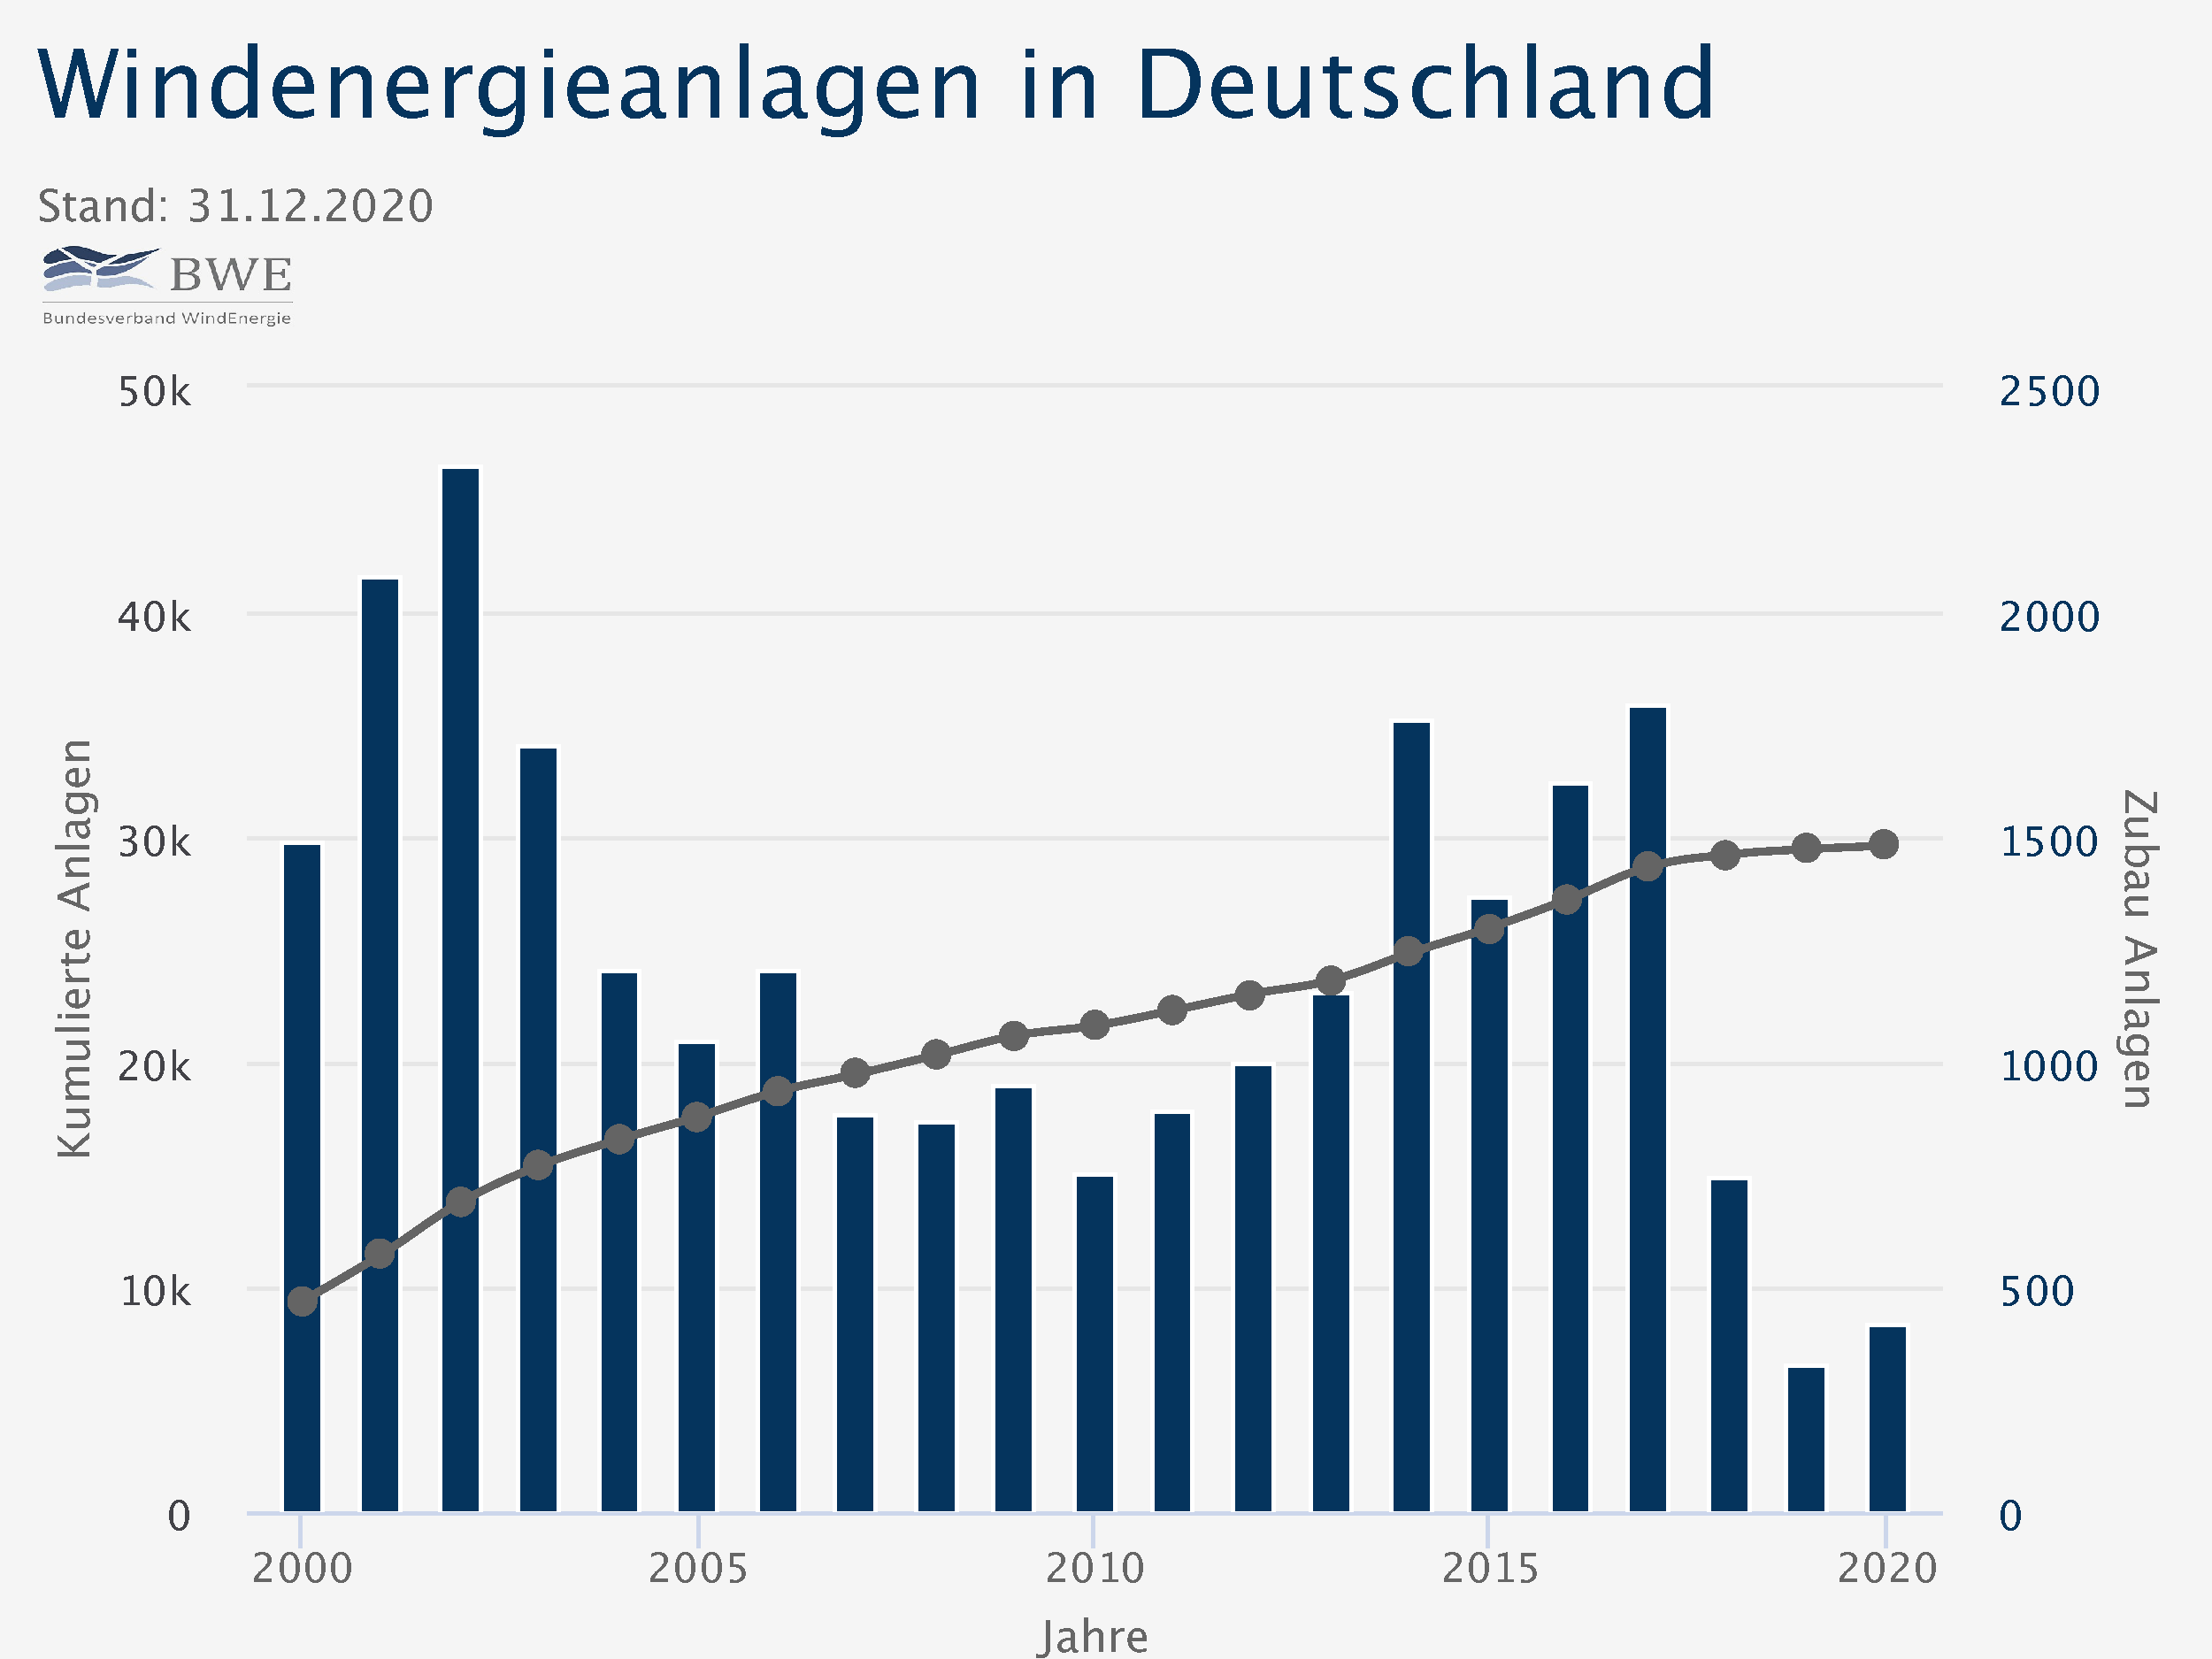
\includegraphics[width=.8\textwidth]{./images/windanlagen_deutschland.pdf}
		\caption{Aktueller Stand der Windkraft in Deutschland; Massiver Rückgang im Zubau in den letzten drei Jahren. \highlight{https://www.wind-energie.de/themen/zahlen-und-fakten/deutschland/ am 19.03.2021}}
		\label{fig:windkraft_deutschland}
	\end{center}
\end{figure}
%%%%%BILD ENDE

\section{Verwandte Literatur}

\highlight{Einige Herangehensweisen Thema Prognose der Windgeschwindigkeit: 
deterministisch (Lorenz), Autoregressive Modelle (ARIMA,SARIMA), Autoregressive Modelle im Mehrdimensionalen (VAR, VARTA), 
Decision Tree,  Neuronale Netze (häufig CNN mit LSTM kombiniert). 
Hierbei waren Lösungsansätze mit letzterem häufig sehr vielversprechend, jedoch auch zahlreich.
Wir grenzen Auswahl anhand uns wichtiger Merkmale ein. 
Uns ist wichtig kurzzeitprognose (stündliche Vorhersage), ähnliche klimatische Bedingungen wie in Deutschland, Beachten und Vorhersage der Windgeschwindigkeit UND Windrichtung (selten in Literatur, meist ausschließlich Geschw.) 
Deswegen etwas genauer: Kreuzer (wegen Deutschlanddaten, NN), USA Paper, Ranganayaki wegen Windrichtung
}

\section{Ziel dieser Arbeit}

\highlight{Aus Einleitung (Windpark Windprognose) und Verwandte Literatur werden Ziele dieser Seminararbeit ersichtlich. 
Mit Daten aus Deutschland (Erwähnte Paper in 1. Hatten ausschließlich Wetterdaten verwendet, dessen Klima stark von kontinentalem Klima abweicht) 
soll mithilfe von Neuronalen Netzen, genauer CNN mit LSTM (erwies sich in Literaturrecherche als guter Ansatz für ähnliche Fragestellungen) ein 
Modell entwickelt werden, welches Windgeschwindigkeit und -richtung stündlich bis zu 24h in die Zukunft prognostizieren kann. 
Um die Güte dieses Modells einordnen zu können, soll mit dem bewährten Modell SARIMA und/oder einem anderen, ähnlichen Modell verglichen werden. 
Der Einfluss von weiteren umliegenden Wetterstationen soll auch berücksichtigt werden.} \\

\highlight{mithilfe mehrerer umliegender Wetterstationen prognostizieren wir für eine Wetterstation}

%%%%%%%%%%%%%%%%%%%%%%%%%%%%%%%%%%%%%%%%%%%%%%%%%%%%%%%%%%%%%%%%%%%%%%%
%                                                                     %
%                                                                     %
%                                                                     %
%                               KAPITEL                               %
%                                                                     %
%                                                                     %
%                                                                     %
%%%%%%%%%%%%%%%%%%%%%%%%%%%%%%%%%%%%%%%%%%%%%%%%%%%%%%%%%%%%%%%%%%%%%%%
\chapter{Grundlagen}

\section{Neuronale Netze zur Zeitreihenprognose}
\highlight{ein paar Grundlagen zu neuronalen Netzen (nicht zu tief gehend): 
Beschreibung versch Architekturen}

\section{Das SARIMA-Modell}
\highlight{Grob SARIMA-Modell erklären. Wenn wir es als Benchmark verwenden}

%%%%%%%%%%%%%%%%%%%%%%%%%%%%%%%%%%%%%%%%%%%%%%%%%%%%%%%%%%%%%%%%%%%%%%%
%                                                                     %
%                                                                     %
%                                                                     %
%                               KAPITEL                               %
%                                                                     %
%                                                                     %
%                                                                     %
%%%%%%%%%%%%%%%%%%%%%%%%%%%%%%%%%%%%%%%%%%%%%%%%%%%%%%%%%%%%%%%%%%%%%%%

\chapter{Implementierung des Modells}

\section{Datenbasis}
\highlight{Blabla über Daten die für Neuronales Netz bla. Vielleicht auch nur was unterschied reale und generierte Daten ist.}

%%%%%BILD ANFANG
\begin{figure}[tph]
	\begin{center}
		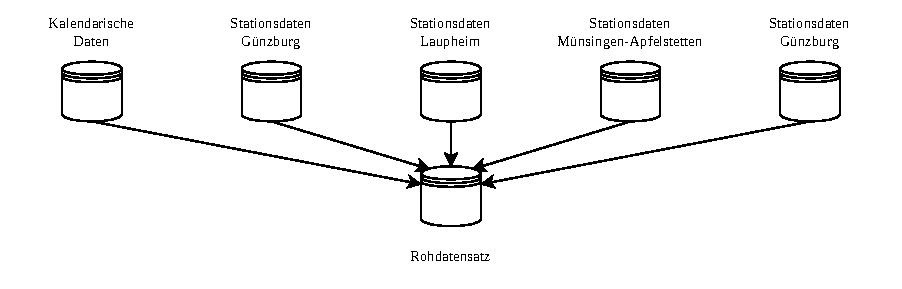
\includegraphics[]{./images/rohdatensatz.pdf}
		\caption{\highlight{{TODO}}}
		\label{fig:rohdatensatz}
	\end{center}
\end{figure}
%%%%%BILD ENDE

\subsection{Reale Messdaten}
\highlight{Daten vom DWD, Windrichtung, -geschwindigkeit (Stundenmittel), Sonnenscheindauer, Druck, Temp, Luftfeuchtigkeit. 
Stündliche Daten im Zeitraum 2008-2021, Wie viele Daten fehlen insgesamt (Maybe Grafik?). 
Tabelle mit Wetterstationen. (plus PLZ oder Kilometer von prognos. Messtation entfernt) . 
Stichwort Windrose.}

%%%%%BILD ANFANG
\begin{figure}[tph]
	\begin{center}
		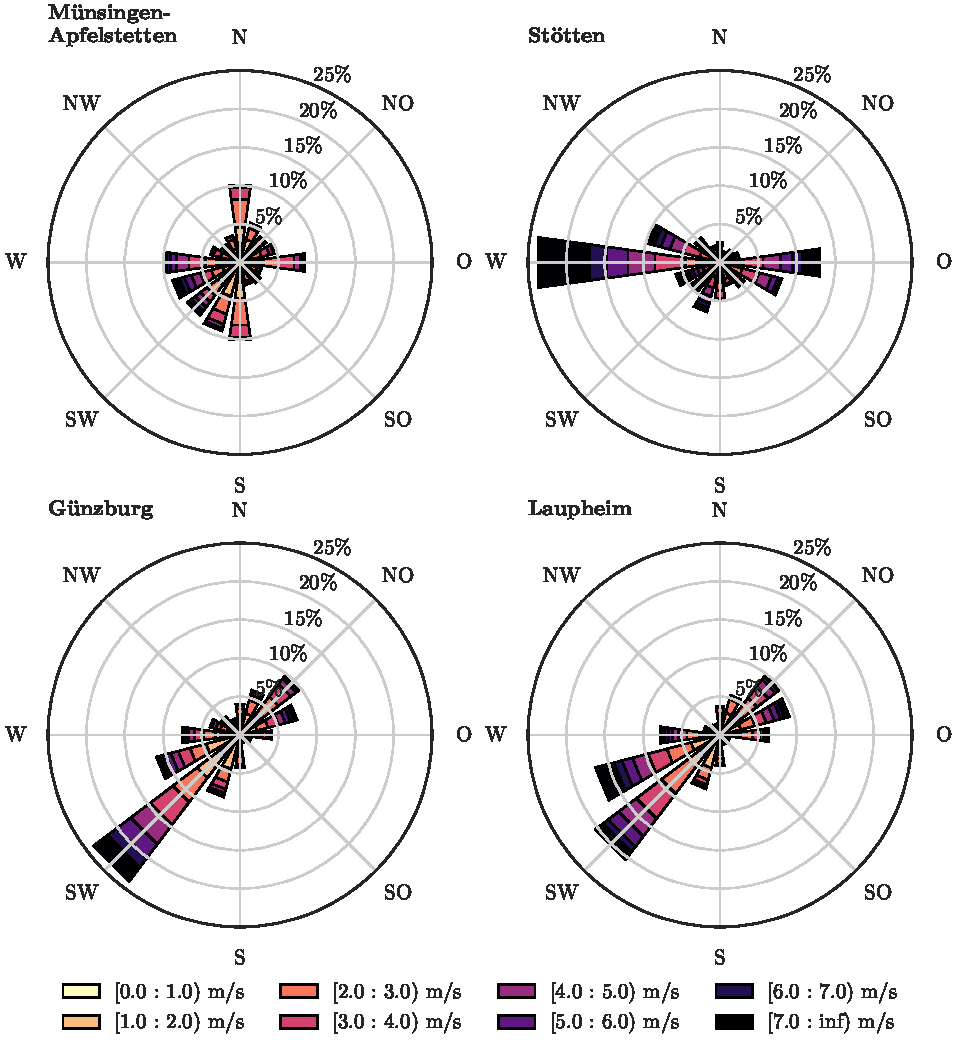
\includegraphics[]{./images/windroses.pdf}
		\caption{\highlight{{TODO}}}
		\label{fig:windroses}
	\end{center}
\end{figure}
%%%%%BILD ENDE

%%%%%BILD ANFANG
\begin{figure}[tph]
	\begin{center}
		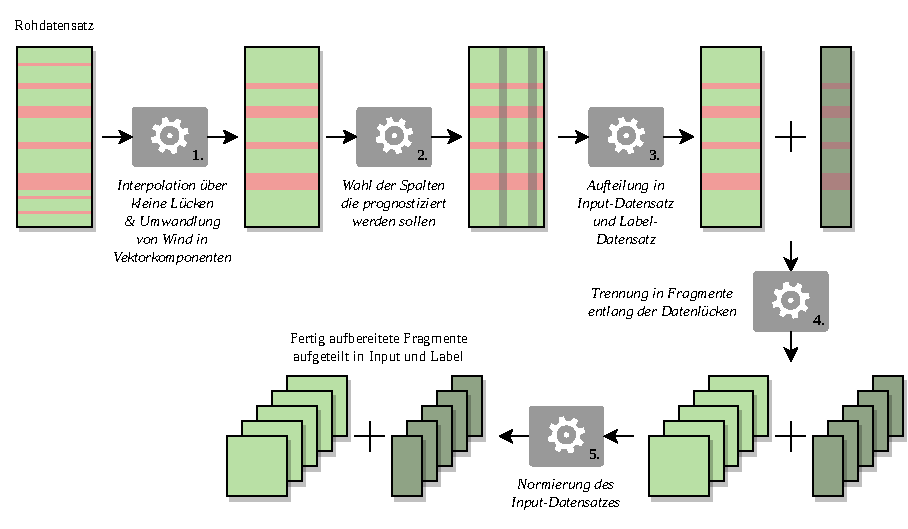
\includegraphics[]{./images/preprocessing.pdf}
		\caption{\highlight{{TODO}}}
		\label{fig:preprocessing}
	\end{center}
\end{figure}
%%%%%BILD ENDE

%%%%%BILD ANFANG
\begin{figure}[tph]
	\begin{center}
		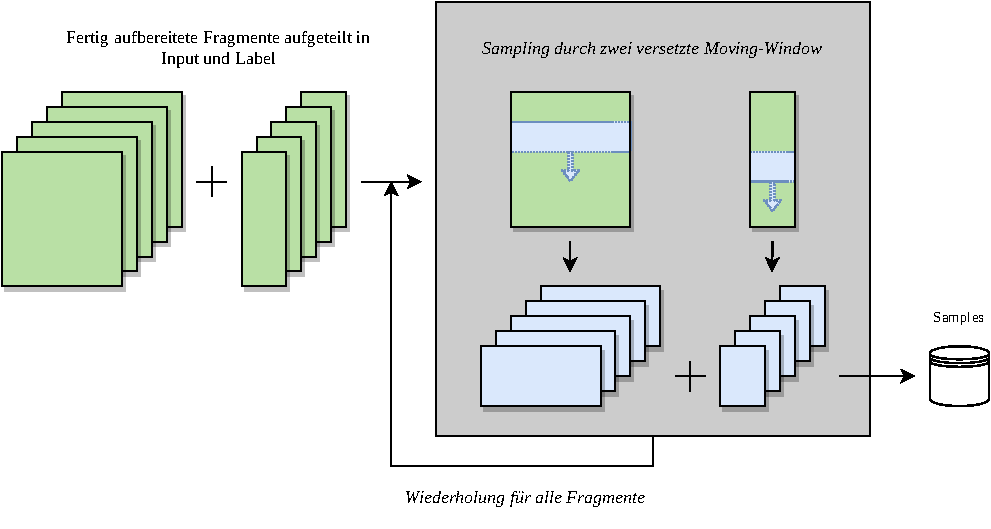
\includegraphics[]{./images/sampling.pdf}
		\caption{\highlight{{TODO}}}
		\label{fig:sampling}
	\end{center}
\end{figure}
%%%%%BILD ENDE

\subsection{Generierte Messdaten}
\highlight{Kalendarische Daten: Tagessinus und Saisonalen Sinus (Korrelationskoeffizienten Wind zu Uhrzeit; Histogramm Uhrzeit und Windverteilung); 
Formeln, kurz Zusammenhang zu Uhrzeit}\\

\highlight{DOY ist DayOfYear und HOD ist HourOfDay; $=$-Zeichen am besten übereinander}

\begin{equation}
	\label{eq:cal_seas}
	cal_{seas,i} = \frac{1}{2}(\cos(\pi (\frac{DOY_i -1 + \frac{HOD_i}{24}}{\frac{365}{2}}+ 1)) + 1)
\end{equation}
\begin{equation}
	\label{eq:cal_day}
	cal_{day,i} = \frac{1}{2}(\cos(\pi (\frac{HOD_i}{12}+ 1)) + 1)
\end{equation}

\section{Datenaufbereitung}
\highlight{hier geht es um die ausgewählten Datensätze, umgang mit Fehldaten, 
Umwandeln der Daten, etc;  
Flowchart über einzelne Schitte der Datenaufbereitung von Roh zu fertige Daten für NN}

\subsection{Winddaten als Vektoren}
\highlight{GRAFIK2 (die von Tensorflow für eine ausgewählte Wetterstation); 
Formulieren wie es geht und formulieren warum (siehe Grafik2) x-y so viel besser sein solte als rad-betrag}

%%%%%BILD ANFANG
\begin{figure}[tph]
	\begin{center}
		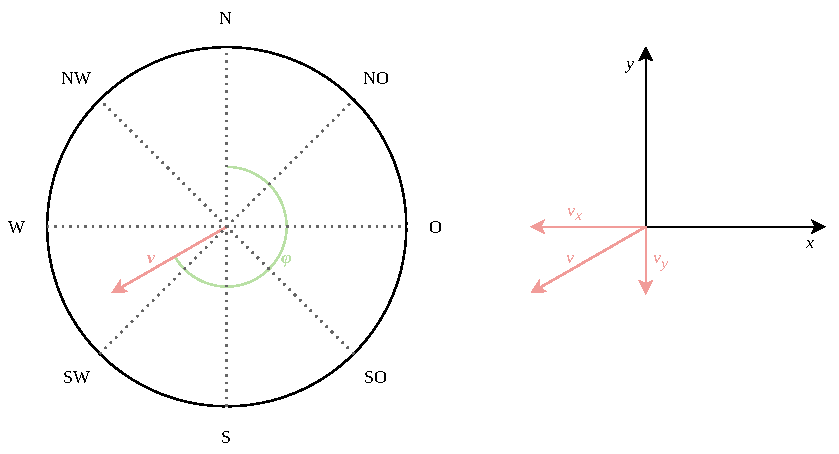
\includegraphics[scale = 1]{./images/pol2cart.pdf}
		\caption{Interpretation der Windgeschwindigkeit und Windrichtung als Vektorkomponenten}
		\label{fig:pol2cart}
	\end{center}
\end{figure}
%%%%%BILD ENDE

%%%%%BILD ANFANG
\begin{figure}[tph]
	\begin{center}
		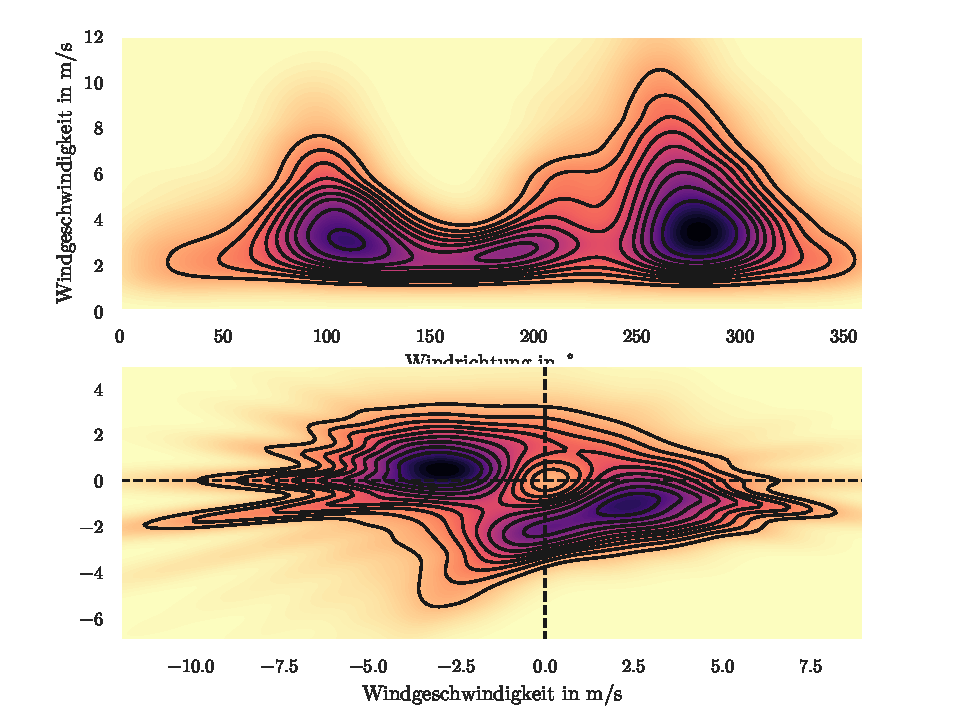
\includegraphics[scale = 1]{./images/pol2cart_visualize.pdf}
		\caption{Verteilung des Windes bei $(v,\phi)$ bzw. $(v_x,v_y)$-Interpretation für die Messtation Ulm-Mähringen im Zeitraum 01.2016 bis 03.2021}
		\label{fig:pol2cart2}
	\end{center}
\end{figure}
%%%%%BILD ENDE

\subsection{Festlegen der In- und Outputs \highlight{(Arbeitstitel)}}
\highlight{Daten in Ein- und Ausgangsdaten trennen: Tabelle sind Eingabedaten (in normalisiert) und zwei Spalten (Windx und Windy) sind Ausgabedaten, aber nicht normalisiert; 
Normalisieren: Mit  Min-Max Normalisierung; Tabelle und nach einzelnen Datenreihen unterscheiden (kalendarisch ausgeschlossen, Wind x-y sind -1 bis 1, damit 0=0)}

%%%%%TABELLE ANFANG
\begin{table}[ht]
	\centering
	\caption{Normalisierung der Eingabedaten}
	\begin{tabular}{|c|c|c|c|c|c|c|c|}
		\hline
		\rowcolor{color80}
		\textbf{$X$}     & \textbf{$w_x$}                 & \textbf{$w_y$}                 & \textbf{$p$}                   & \textbf{$T$}                   & \textbf{$RH$}                  & \textbf{$cal_{day}$} & \textbf{$cal_{seas}$} \\ \hline
		Einheit X      & $m/s$                          & $m/s$                          & $hPa$                          & $^\circ C$                      & \%                            & 1                    & 1                     \\ \hline
		$min(X)$       & \highlight{?} & \highlight{?} & \highlight{?} & \highlight{?} & \highlight{?} & 0                    & 0                     \\ \hline
		$max(X)$       & \highlight{?} & \highlight{?} & \highlight{?} & \highlight{?} & \highlight{?} & 1                    & 1                     \\ \hline
		$min(norm(X))$ & -1                             & -1                             & 0                              & 0                              & 0                              & -                    & -                     \\ \hline
		$max(norm(X))$ & 1                              & 1                              & 1                              & 1                              & 1                              & -                    & -                     \\ \hline
	\end{tabular}
\label{tab:normalisierung}
\end{table}
%%%%%TABELLE ENDE


\subsection{Datenlücken}
\highlight{Zeitreihen separat angeschaut (Spaltenweise Lücken interpoliert/korrigiert (Nur eine Art Daten angesehen, wie z.B. Temperatur nur mit umliegenden Temperaturdaten verglichen) 
Maximale Lücke 4 Stunden (wurde noch linear interpoliert); 
Jetzt sind nur noch größere Lücken als 4 Stunden im Datensatz, wir teilen entlang dieser großen Lücken unsere Tabelle in kleinere Tabellen (chunks), keine Fehldaten mehr :)}

\subsection{Sampling \highlight{(Arbeitstitel)}}
\highlight{Grafik um das Verschieben zu visualisieren; chunks werden der Reihe nach durchlaufen; 
innerhalb chink wird über ein moving window gesampelt; Ein- und Ausgabefesnter sind verschoben (zeitlich); 
Details: wie lange sind die Fenster, wie hoch, Größendefinition, bla}

\subsection{Datenaufteilung \highlight{(Arbeitstitel)}}
\highlight{Blabla dass man Daten in drei Teile für NN teilt, warum das wichtig ist, bla; 
Wie viele Samples haben wir? Aufteilung in Trainings (65\%), Validierungs(30\%) und Testdaten (5\%)}

\section{Implementierung SARIMA und/oder anderes Vergleichsmodell}
\highlight{Hier ist Platz für alles, was mit der implementierung des Vergleichsmodells zu tun hat. 
alles bis auf Ergebnisse}

\section{Entwicklung und Trainieren des Neuronalen Netzes}
\highlight{Hier ist Platz für alles, was mit der implementierung des eigentlichen Modells zu tun hat. 
Infos zu den Layers, zum Trainingsvorgang, Das mit den Decision Trees zur Auswahl der besten Paramter, 
alles bis auf Ergebnisse}

\subsection{Festlegung der Modellarchitektur \highlight{(Arbeitstitel)}}
\highlight{Begründen aus welchen Gründen wir uns für diese drei Methoden entschieden haben 
(RNNseq2seq, RNNseq2vec, DNN) z.B. Datengrundlage, Zeitaspekt, bla; 
Tabelele: Welche Lossfunktion, Metric, Prognosehorizont, Historie, tatsächliche Architektur (Schichten, Neuronen), 
welche Regularisierung + dazu immer etwas schreiben }

\subsection{Trainingsphase}
\highlight{Random search über Konfigurationen aus Tabelele und daraus optimales NN, hierüber schreiben; 
optionale Grafik über Fehler, Loss, und so}

\section{Ergebnisse}
\highlight{Hier nur die Ergebnisse zeigen und nüchtern darauf eingehen. Diskussion kommt ein Kapitel später. Einige Grafiken.}

%%%%%%%%%%%%%%%%%%%%%%%%%%%%%%%%%%%%%%%%%%%%%%%%%%%%%%%%%%%%%%%%%%%%%%%
%                                                                     %
%                                                                     %
%                                                                     %
%                               KAPITEL                               %
%                                                                     %
%                                                                     %
%                                                                     %
%%%%%%%%%%%%%%%%%%%%%%%%%%%%%%%%%%%%%%%%%%%%%%%%%%%%%%%%%%%%%%%%%%%%%%%

\chapter{Diskussion und Ausblick}
\highlight{Oben gezeigten Ergebnisse werden verglichen und die Ergebnisse anhand von Fehlermaß und Vergleich mit anderem Ansatz diskutiert ;
Später noch Ausblick bla}

\section{Diskussion der Ergebnisse}
\highlight{Was auch immer wir herausbekommen. In Kontext setzen. War unser Modell vergleichsweise gut? Hier vll auch 
Diskussion über Unterschied zwischen eine und mehrere Wetterstationsdaten.}

\subsection{Vergleich der entwickelten Modelle}
\highlight{Fehler (RMSE, MAE) anschauen und interpretieren der unterschiedlichen Netze; 
Fehler pro Windgeschwindigkeit; Fehler über Prognosehorizont}

\subsection{Einfluss kartesischer Winddaten}
\highlight{Vergleich kartesisch und polar am besten Modell}, wieder auf Grafik oben eingehen

\subsection{Einordnung in existierenden Prognosemodellen \highlight{(Arbeitstitel)}}
\highlight{entweder SARIMA oder ein anderes Netz aus Paper (zB Amerika oder so) verwenden und grob vergleichen der Fehler und erklären, dass
 Klima ähnlich und deswegen eher vergleichbar, aber nicht absolute Sicherheit!!! (Geht über Umfang der arbeit hinaus)}

\section{Weiterentwicklung des Modells}
\highlight{Das ist der Ausblick. Was könnte man noch tolles anstellen wo wir aber keine Zeit mehr für hatten? Idee Ensemble-Modell, andere Daten 
verwenden, um Modell besser mit anderem bestehendem zu Vergleichen, Satellitendaten einbinden, weitere Modelle untereinander vergleichen mit Ulmer Klimadaten}

%%%%%%%%%%%%%%%%%%%%%%%%%%%%%%%%%%%%%%%%%%%%%%%%%%%%%%%%%%%%%%%%%%%%%%%
%                                                                     %
%                                                                     %
%                                                                     %
%                               KAPITEL                               %
%                                                                     %
%                                                                     %
%                                                                     %
%%%%%%%%%%%%%%%%%%%%%%%%%%%%%%%%%%%%%%%%%%%%%%%%%%%%%%%%%%%%%%%%%%%%%%%
\chapter{Test und Wissen}

\section{Tabelle}
%%%%%TABELLE ANFANG
\begin{table}[ht]
	\centering
	\caption{Das hier ist eine Testtabelle, man beachte die gezwungene Breite in der rechten Spalte. Lässt sich einfach durch den Befehl C\{5cm\} erzeugen.}
	\begin{tabular}{|l|C{5cm}|}
		\hline
        \rowcolor{color80}
		\textbf{Erste Zelle}&\textbf{Ein Header}\\
		\hline
		Moin: & Zusammen\\\hline
		leer:&\\\hline
		Moin: & Zusammen\\\hline
		leer:&\\\hline
	\end{tabular}
\label{tab:testtabelle}
\end{table}
%%%%%TABELLE ENDE

%%%%%LANGTABELLE ANFANG
\begin{longtable}{|L{3.6cm}|L{6cm}|L{6cm}|}
	\caption{Finale Merkmale}\label{tab:longtable}\\
    % Definition des Tabellenkopfes auf der ersten Seite
	\hline
    \rowcolor{color80}
	\textbf{Abkürzung}&\textbf{Englisch}&\textbf{Deutsch}\\
	\hline
	\endfirsthead % Erster Kopf zu Ende
	% Definition des Tabellenkopfes auf den folgenden Seiten
	\hline
	\rowcolor{color80}
	\textbf{Abkürzung}&\textbf{Englisch}&\textbf{Deutsch}\\
	\hline
	\endhead % Zweiter Kopf ist zu Ende
    \hline
    \endfoot
    \hline
    \endlastfoot
	% Ab hier kommt der Inhalt der Tabelle
	$test_{\mathrm{abk}}$&ein sehr sehr sehr langertextmit langen wörternein sehr sehr sehr langertextmit langen wörternein sehr sehr sehr langertextmit langen wörternein sehr sehr sehr langertextmit langen wörternein sehr sehr sehr langertextmit langen wörtern&Einzeilig\\
	Z&5&as\\\hline
	A&1&91\\\hline
	B&2&97\\\hline
	Z&5&as\\\hline
	A&1&91\\\hline
	B&2&97\\\hline
	A&1&91\\\hline
	B&2&97\\\hline
	Z&5&as\\\hline
	A&1&91\\\hline
	B&2&97\\\hline
    Z&5&as\\\hline
	A&1&91\\\hline
	B&2&97\\\hline
	Z&5&as\\\hline
	A&1&91\\\hline
	B&2&97\\\hline
    Z&5&as\\\hline
	A&1&91\\\hline
	B&2&97\\\hline
	Z&5&as\\\hline
	A&1&91\\\hline
	B&2&97\\\hline
    Z&5&as\\\hline
	A&1&91\\\hline
	B&2&97\\\hline
	Z&5&as\\\hline
	A&1&91\\\hline
	B&2&97\\\hline
    Z&5&as\\\hline
	A&1&91\\\hline
	B&2&97\\\hline
	Z&5&as\\\hline
	A&1&91\\\hline
	B&2&97\\\hline
    Z&5&as\\\hline
	A&1&91\\\hline
	B&2&97\\\hline
	Z&5&as\\\hline
	A&1&91\\\hline
	B&2&97\\\hline
	Z&5&as\\\hline
	A&1&91\\\hline
	B&2&97\\\hline
	Z&5&as\\\hline
	A&1&91\\\hline
	B&2&97\\\hline
	Z&5&KEINE hline AMSCHLUSS!!!\\
\end{longtable}
%%%%%LANGTABELLE ENDE

\section{Bild}

%%%%%BILD ANFANG
\begin{figure}[tph]
	\begin{center}
		
\includegraphics[scale = 1]{./images/0_testbild.png}
		\caption{TEST Hier ist ein wunderschönes Testbild zu erkennen, und das hier ist ein wunderschönes Testbild zu erkennen, und das hier ist ein wunderschönes Testbild zu erkennen, und das hier ist ein wunderschönes Testbild zu erkennen, und das hier ist ein wunderschönes Testbild zu erkennen, und das hier ist ein wunderschönes Testbild zu erkennen, und das hier ist ein}
		\label{fig:testbild}
	\end{center}
\end{figure}
%%%%%BILD ENDE

%%%%%DOPPELBILD ANFANG
\begin{figure}
	\centering
	\begin{minipage}[b]{.4\linewidth} % [b] => Ausrichtung an \caption
		
\includegraphics[width=\linewidth]{./images/0_testbild.png}
		\caption{Beschreibung und so}
		\label{fig:testbild_klein_links}
	\end{minipage}
	\hspace{.1\linewidth}% Abstand zwischen Bilder
	\begin{minipage}[b]{.4\linewidth} % [b] => Ausrichtung an \caption
		
\includegraphics[width=\linewidth]{./images/0_testbild.png}
		\caption{Zweite Beschreibung}
		\label{fig:testbild_klein_rechts}
	\end{minipage}
\caption*{Hier steht eine etwas längere Bildunterschrift, die dieses Doppelbild beschreibt. Zu sehen sind weder Land noch Wasser, das macht bei Testbildern aber nix.}
\end{figure}
%%%%%DOPPELBILD ENDE

\section{Formeln}

Aufpassen, hier kommt jetzt eine einfache Testformel hin:

\begin{equation}
\label{eq:1}
x=10
\end{equation}

Diese Formel \autoref{eq:1} kann auch referenziert werden.

\begin{equation}
x=Ma_{\mathrm{blabla}} \cdot y
\end{equation}

\section{Zitate}

Um Bib zu kompilieren, einmal F8 drücken.

Bild \autoref{fig:testbild} referenzieren.
%Auch ein Autorname \citeauthor{ernstGrundkursInformatikGrundlagen2015} oder ein Jahr geht \citeyear{ernstGrundkursInformatikGrundlagen2015}

%%%%%%%%%%%%%%%%%%%%%%%%%%%%%%%%%%%%%%%%%%%%%%%%%%%%%%%%%%%%%%%%%%%%%%%
%                                                                     %
%                                                                     %
%                                                                     %
%                               KAPITEL                               %
%                                                                     %
%                                                                     %
%                                                                     %
%%%%%%%%%%%%%%%%%%%%%%%%%%%%%%%%%%%%%%%%%%%%%%%%%%%%%%%%%%%%%%%%%%%%%%%
\chapter{Quellen}
\end{document}